\documentclass[journal]{IEEEtran}

\ifCLASSINFOpdf
\else
   \usepackage[dvips]{graphicx}
\fi
\usepackage{url}

\hyphenation{op-tical net-works semi-conduc-tor}

\usepackage{graphicx}
\usepackage[utf8]{inputenc} 
\usepackage[T1]{fontenc}
\usepackage{url}
\usepackage{bm}
\usepackage[cmex10]{amsmath} 
\usepackage{ifthen}
\usepackage{cite}
\usepackage{color}
\usepackage{graphicx}
\usepackage{amssymb}
\usepackage{amsthm}
\usepackage{amsfonts}
\usepackage{comment}
\usepackage[utf8]{inputenc} 
\usepackage[T1]{fontenc}
\usepackage{url}
\usepackage{ifthen}
\usepackage{cite}
\usepackage{color}
\usepackage{graphicx}
\usepackage{amssymb}
\usepackage{amsthm}
\usepackage{amsfonts}
\usepackage{comment}

\usepackage[skip=5pt,style=base]{caption}

\usepackage{bm}
\usepackage[cmex10]{amsmath} % Use the [cmex10] option to ensure complicance
                             % with IEEE Xplore (see bare_conf.tex)

%% Please note that the amsthm package must not be loaded with
%% IEEEtran.cls because IEEEtran provides its own versions of
%% theorems. Also note that IEEEXplore does not accepts submissions
%% with hyperlinks, i.e., hyperref cannot be used.

\interdisplaylinepenalty=2500 % As explained in bare_conf.tex
%%%%%%
% correct bad hyphenation here
\hyphenation{op-tical net-works semi-conduc-tor}
\DeclareMathOperator{\E}{\mathbb{E}}
\DeclareMathOperator{\C}{\mathbb{C}} 
\newcommand{\argmax}{\operatornamewithlimits{argmax}}
\newcommand{\argmin}{\operatornamewithlimits{argmin}}
\newcommand{\zz}[1]{\textsf{\textbf{\color{red}{\tiny [ZZ: #1]}}}}
\newcommand{\pp}[1]{\textsf{\textbf{\color{green}{\tiny [P: #1]}}}}
\DeclareMathOperator{\Tr}{Tr}
\usepackage[skip=5pt,style=base]{caption}
%\doublespacing
\begin{document}
\title{Constrained graph-based model selection in multi-modal switching linear dynamic systems}

% \IEEEmembership{Member}|

\author{Parisa Karimi, Mark Butala, and Farzad Kamalabadi
\thanks{This work was supported by the Grainger college of engineering UIUC-ZJU institute.}
\thanks{P.Karimi$^*$, and F.Kamalabadi are with the University of Illinois at Urbana-Champaign, Urbana, IL. 61801, USA (e-mail$^*$: parisa2@illinois.edu).}
\thanks{M.Butala is with the Zhejiang University, Hangzhou, Zhejiang, P.\ R.\ China.}}
% \thanks{The next few paragraphs should contain the authors’ current affiliations, including current address and e-mail. For example, F. A. Author is with the National Institute of Standards and Technology, Boulder, CO 80305 USA (e-mail: author@boulder.nist.gov).}
% \thanks{S. B. Author, Jr., was with Rice University, Houston, TX 77005 USA. He is now with the Department of Physics, Colorado State University, Fort Collins, CO 80523 USA (e-mail: author@lamar.colostate.edu).}}

\markboth{IEEE Signal Processing Letters, June 2020}
{Shell \MakeLowercase{\textit{et al.}}: Bare Demo of IEEEtran.cls for IEEE Journals}
\maketitle
\begin{abstract}
Switching Kalman Filters (SKF) are well known for their ability to solve the switching linear dynamic system (SLDS) estimation problem using multiple standard Kalman Filters (KF). The computational resources required for the optimal SKF increases exponentially with the number of modes, and even the heuristic, approximate SKFs require significantly more computational resources than a single-mode KF when the state dimension is large. The goal of this paper is to find the best set of switching modes for estimation in an SLDS given specific computational constraints. This goal is obtained by proposing a graph structure for the SLDS. By clustering the modes, one can answer important questions including what is the best set of modes given an error tolerance or what is the best set of modes given an upper bound for the number of modes. Applying the proposed algorithm to problems where a set of dynamic systems are a priori given or learned from the data using batch/real time system identification algorithms will result in gaining computational benefit at the cost of accepting an error tolerance in estimation.
\end{abstract}
\begin{IEEEkeywords}
Switching linear dynamic systems, Switching Kalman filter, recursive estimation, model mismatch.
\end{IEEEkeywords}
\IEEEpeerreviewmaketitle

\vspace{-.5cm}
\section{Introduction}

\IEEEPARstart{A}{} pervasive problem in virtually all branches of physics and engineering sciences, such as time-dependent tomography and imaging \cite{rem1,rem2}, geophysical data assimilation \cite{geo}, genetics \cite{gene}, and economic forecasting \cite{eco}, is the estimation of multi-dimensional state variables of a dynamical system from a collection of indirect, noisy measurements. Given the initial state distribution and a state-space model, state estimates may be recovered using Bayesian inference algorithms \cite{bayes}. The Kalman filter \cite{kalman} provides the optimal solution for the linear state space equation with additive Gaussian noise\cite{lin}.  %Nevertheless, the full potential and wide-spread application are restricted by the inherent assumptions of the underlying models; these assumptions are the motivation for the existence of many different inference algorithms. 


% Many algorithms have been proposed in the Bayesian framework to solve the estimation problem, ranging from non-parametric models \cite{nonp}  (assuming to have no prior information about the underlying model) to parametric models (where we assume to know the underlying evolution and observation models). For specific applications, the state evolution and measurement distribution may be regarded as static for each measurement, and the assumptions of linearity and Gaussian noise may be reasonable. The Kalman Filter \cite{kalman} (KF) can update unbiased estimates of the state’s mean and covariance in an optimal sense, assuming linear dynamics and Gaussian noise. However, in many applications, these assumptions are not realistic. Monte Carlo filters, such as the particle filter \cite{particle} may solve problems with arbitrary models based on importance sampling. However, they are not desirable in the online estimation of high dimensional state parameters due to their high computational costs.

% The , which results in a
% Different Dynamic Bayesian networks (DBN) may be used as representative models of a dynamic system .
A computationally efficient generalization of the linear state-space model is obtained by augmenting hidden discrete random variables to the linear model to account for nonlinearities, referred to as a switching linear dynamic system (SLDS) \cite{dbn}. In an SLDS, random switches occur in the system’s dynamic model, and Bayesian estimation may be used to estimate both the discrete modes and continuous states using switching Kalman filters(SKF)\cite{skf,skf2,skf3}; dynamic systems such as financial time series and brain electrical activity may be represented using these parameterized models\cite{fin,eeg}. The computational complexity of the SKF directly depends on the cardinality of the set of switching modes\cite{skf3}. On the other hand, if the switching modes are not distant enough (i,e. in KL divergence sense), applying a SKF will not have a significant impact on the estimation error since the conditional distributions of the modes will be very similar, the detection error using a likelihood ratio test will be large, and the estimation error caused by using mismatched stochastic models will be small[our SPL paper]. Therefore, choosing a set of effective modes given computational constraints becomes a problem of great importance, specially in high dimensional problems.



The main assumption of this work is that the set of switching linear dynamic models are given; In practice, this set is usually learned from the data using online/batch system identification algorithms.(is the rest of this paragraph necessary?) Many algorithms have been proposed to perform system identification in switching systems including algebraic approaches \cite{si_alg,si-alg2,sis-alg3} and Bayesian algorithms \cite{si-bay,hdp}. Online system identification algorithms, assuming a minimum dwell time for the modes, usually use two stage algorithms to detect the segments of data with the same dynamic evolution parameters and learning/updating these parameters \cite{sis-on1,sis-on2,sis-on3}



This paper proposes a systematic way to represent and characterize an SLDS using a fully connected graph, where a node represents one subset of parameters for the SLDS (switching modes) and an edge between two nodes is a measure based on the estimation error caused by mismatch if one uses one node's parameters instead of the other one calculated in terms of mean squared error (MSE); this measure is calculated based on the derived error metric in [SPL paper]. Then, by applying a clustering algorithm to this graph, one is able to reduce the computational complexity of state estimation while maintaining an acceptable error tolerance. Also, one is able to quantify the effect of each mode in an SLDS in terms of estimation error based on this representation. To reduce the computational burden of building this graph, the authors propose to use a partially connected graph, which will be presented in another publication. The simulation results study a physics-motivated diffusion problem with multiple switching modes; clustering the modes using the graph structure provides a significant improvement in computation while losing a tolerable amount of accuracy in estimation. 



The remainder of the paper is organized as follows. The common notations used throughout the paper are presented in section \ref{section:not}. The SLDS signal model and KF/SKF formulations are reviewed in Sections \ref{section:slds} and \ref{section:skf}, respectively. Section \ref{section:error} derives estimation error for mismatched KFs and SKFs in SLDS and \ref{section:graph} introduces the graph structure. Simulations verify the derivations in Section~\ref{section:sim}, and conclusions are presented in Section~\ref{section:con}. 



\section{Notation}\label{section:not}
\begin{itemize}
    \item $\bm{x}\sim N(\bm{m},\bm{C})$: the random vector $\bm{x}$ has a Gaussian distribution with mean $\bm{m}$ and covariance $\bm{C}$.
\item $\E,\C,p$ refer to expectation, covariance, and probability, respectively, and $\bm{I}$ refers to the identity matrix. 
 \end{itemize}
 \vspace{-.55cm}
\section{Signal model}\label{section:slds}
The state-space model for an SLDS may be defined as
\begin{align}
    \bm{x}_n &= \bm{A}_n \bm{x}_{n-1}+\bm{\nu}_n, \label{eqn:sp1}\\
    \bm{y}_n &= \bm{H}_n\bm{x}_n +\bm{\omega}_n \label{eqn:sp2},
\end{align}
where the subscript $n$ is the time step, $\bm{x}_n$ is the hidden state variable to be estimated, and the given model parameters are the measurement vector $\bm{y}_n$, the $z\times z$ evolution matrix $\bm{A}_n \in \{ \bm{A}^{(S_n)}\}, S_n=1,...,r$ ($S_n$ is the hidden random variable determining the mode of the system, to be detected), the $m\times z$ measurement matrix $\bm{H}_n$, and $\bm{Q}_n$ and $\bm{R}_n$ where $\bm{\nu}_n \sim N(0,\bm{Q}_n)$, $\bm{\omega}_n \sim N(0,\bm{R}_n)$ such that $\E[\bm{\nu}_n\bm{\nu}_{n'}^T]=\bm{Q}_n\,\delta(n-n')$, $\E[\bm{\omega}_n\bm{\omega}_{n'}^T]=\bm{R}_n\,\delta(n-n')$, and $\E[\bm{\omega}_n\bm{\nu}_{n'}^T]=\bm{0}$ ($m$ is the number of measurements, $z$ is the state dimension, and $r$ is the number of modes the system may switch between). 
\section{Kalman filter/Switching Kalman filter}\label{section:skf}
 The KF provides an optimal estimator for a linear dynamic system. Let $\bm{y}_1^n\equiv [\bm{y}_1,\bm{y}_2,...,\bm{y}_n]$, $\bm{x}_0\sim N(\bm{x}_{0|0},\bm{P}_{0|0})$, and $\bm{x}_{n|n}=\E[\bm{x}_n|\bm{y}_1^n],\bm{P}_{n|n}=\C(\bm{x}_n|\bm{y}_1^n)$. The "$Filter$" operator is then defined as
\begin{multline}
    (\bm{x}_{n|n},\bm{P}_{n|n}) = Filter(\bm{A}_n,\bm{H}_n,\bm{x}_{n-1|n-1},\bm{P}_{n-1|n-1}, \\ \bm{Q}_n,\bm{R}_n,\bm{y}_1^n), \label{eqn:filter}
\end{multline}
which involves the repeated application of a time update step
%\noindent\textbf{Step 1: Time update equations}
\begin{align}
\bm{x}_{n|n-1} &= \bm{A}_n \bm{x}_{n-1|n-1}, \label{eqn: Kalman1}\\
\bm{P}_{n|n-1}&= \bm{A}_n \bm{P}_{n-1|n-1}\bm{A}_n^T + \bm{Q}_n;
\end{align}
and a measurement update step
%\noindent\textbf{Step 2: Measurement Update equations}
\begin{align}
\bm{\epsilon}_n &= \bm{y}_n - \bm{H}_n \bm{x}_{n|n-1}, \\
\bm{B}_n &= \bm{H}_n \bm{P}_{n|n-1} \bm{H}_n^T + \bm{R}_n,\\
\bm{K}_n &= \bm{P}_{n|n-1} \bm{H}_n^T \bm{B}_n^{-1},\\
% L_n &= N(\bm{\epsilon}_n; \bm{0}, \bm{B}_n),\\
\bm{x}_{n|n} &= \bm{x}_{n|n-1} + \bm{K}_n \bm{\epsilon}_n,\\
\bm{P}_{n|n} &= (\bm{I} - \bm{K}_n \bm{H}_n) \bm{P}_{n|n-1}. \label{eqn:Kalmanend} 
%V_{i,i-1|i}&=(I-K_iH_i)F_iV_{i-1|i-1}
\end{align}
% \section{Switching Kalman Filter}\label{section:skf}
  The application of a single-mode KF to the general SLDS of \eqref{eqn:sp1}-\eqref{eqn:sp2} results in erroneous estimates. The well known SKF formulation detects the switching mode and its corresponding model parameters ($\bm{A}_n,\bm{Q}_n$) at each time step, and estimates the state variables accordingly. Upon perfect detection of the modes, one could obtain optimal estimation of the state variable $\bm{x}_n$ in terms of both MAP and MSE metrics. Due to the exponentially exploding nature of the posterior in optimal SKFs\cite{SKF}, several approximate SKF algorithms have been proposed (i.e. \cite{SKF,imm}). Due to space restrictions, we assumed an estimate of the detection rate to be known and the details of the approximate SKF algorithms are not presented here. 
%  However, in a SKF formulation, detection is not perfect. In other words, detection error affects the estimation error and estimation error affects the detection error. 

%  \begin{multline}
%  (\bm{x}_{n|n}^{i,j},\bm{P}_{n|n}^{i,j},L_n^{i,j} )=Filter(\bm{A}^{j},\bm{x}_{n-1|n-1}^i,\bm{P}_{n-1|n-1}^i, \\ \bm{Q}_n^{j},\bm{R}_n^{j},\bm{y}_1^n), \label{eqn:skf_filter}
% % &\bm{x}_{t|\tau}^{i(j)} =E[\bm{x}_t|\bm{y}_{1:\tau},S_{t-1} = i , S_t=j]\\
% % &\bm{P}_{t|\tau}^{i(j)}   =Cov[\bm{X}_t|\bm{y}_{1:\tau},S_{t-1} = i , S_t=j]\\
% % &M_{t|\tau}(j) = Pr(S_t=j|\bm{y}_{1:\tau})\\
% % &M_{t-1,t|\tau}(i,j) = Pr(S_{t-1}=i,S_t=j|\bm{y}_{1:\tau})\\
% % &L_t^{i(j)} = Pr(\bm{y}_t|\bm{y}_{1:t-1},S_{t-1}=i,S_t = j)\\
% % &Z= \text{Probability transition matrix of the indicator variable}
% \end{multline}
% where $i$ refers to the previous mode and $j$ refers to the current mode of the system. Assuming a bi-modal system, the mode detection procedure is as follows: 
% % \begin{align}
% %     &argmax_{x_n} P(x_n|y_1^n) = argmax_{x_n}\int P(x_n,x_{n-1}|y_1^n)dx_{n-1}\\
% %     &=argmax_{x_n}\int \frac{P(y_n|x_n)P(x_n|x_{n-1})P(x_{n-1})dx_{n-1}}{P(y_n|y_1^{n-1})}
% % \end{align}
% % \begin{align}
% %     &argmax_{s_n}P(x_n|x_{n-1}) = argmax_{s_n}\sum_{s_n}  P(x_n,s_n|x_{n-1}) \\
% %     &=argmax_{s_n}\sum_{s_n}  P(x_n|s_n,x_{n-1}) P(s_n|x_{n-1})\\
% %     &=Normaliz(P(x_n|s_{max},x_{n-1}))
% % \end{align}
% \begin{align*}
% S_n &= \argmax\left( \sum_i\pi(i)\bm{Z}(i,1)\bm{L}_{n|n}^{i,1},\nonumber \sum_i\pi(i)\bm{Z}(i,2)\bm{L}_{n|n}^{i,2} \right), %\label{eqn:skfLRT}\\
% % &\bm{x}_{n|n} = \bm{x}_{n|n}^{S_n},\label{eqn:skfmean}\\
% % &\bm{P}_{n|n} = \bm{P}_{n|n}^{S_n}\label{eqn:skfcov}, 
% \end{align*}
% where $S_n$ is the mode of the system at time $n$, $\pi(i)$ is the prior on mode $i$, and $\bm{Z}$ is the transition matrix for the Markov process of mode switches such that $\bm{Z}(i,j)=p(S_n=j|S_{n-1}=i)$. The state estimates at each time are calculated based on the detected modes in the likelihood test. 
% \subsection{Different approximations of SKF: MAP - ML - MMSE}
% \subsection{Detectability of modes : Separation of switching distributions}
% *** Study the bias mean and cov as a function of separation of modes 
% \section{Cramer Rao bound for switching systems}
% \section{Approximate unbiased single linear estimator}\label{section:best}
% The single unbiased filter applied at each time step in a SLDS is referred to as the average filter, where $\bm{A}_n = \pi_1 \bm{A}_1 + \pi_2 \bm{A}_2$ and $\pi_i$ is the probability of mode $i$ at each time. It is trivial to show that given $\bm{x}_{n-1}$ and $\bm{P}_{n-1}$, the average filter always provides unbiased estimates since $\E[\bm{x}_n-\hat{\bm{x}}_n]=\bm{0}$. Considering multiple time steps, the estimator is approximately unbiased as only one time step trajectory is propagated in calculations (a necessary simplification as it is infeasible to propagate all trajectories). Intuitively, if the switching distributions are very close to each other (if $\bm{A}_1=\bm{A}_2$ in the extreme case), the average filter’s estimates are very close to the optimal solution. Alternatively, if the distributions are far from each other (if $\bm{A}_1=-\bm{A}_2$ in an extreme case), the average filter’s estimates are poor. Therefore, this filter is used as a representative of the class of single KFs. 
% An ongoing work of the authors focuses on finding the best single linear KF for a SLDS based on the prior switching information. 


%  \bold{(Can we show that using the average KF is better than always using one of the modes? )}; In order to study this, we need to study the optimal filter at first, which is obtained as 
%  \begin{align}
%      \bm{x}_{opt} = \E[\bm{x}_n|\bm{y}_n] = \sum \pi_i \bm{x}_{n|n}^{d(i)}
%  \end{align}
% therefore, we can study the difference of the estimations from the optimal solution as
% \begin{align}
%     |\bm{x}_{opt}-\bm{x}_1|&=|\pi_2[(\bm{A}_2-\bm{A}_1+\bm{K}_1\bm{H}\bm{A}_1-\bm{K}_2\bm{H}\bm{A}_2)\bm{x}_0\nonumber \\ 
%     &\quad \quad +(\bm{K}_2-\bm{K}_1)\bm{y}]|\\
%     |\bm{x}_{opt}-\bm{x}_2|&=|\pi_1[(\bm{A}_1-\bm{A}_2+\bm{K}_2\bm{H}\bm{A}_2-\bm{K}_1\bm{H}\bm{A}_1)\bm{x}_0\nonumber \\ 
%     &\quad \quad +(\bm{K}_1-\bm{K}_2)\bm{y}]|\\
%     |\bm{x}_{opt}-\bm{x}_{avg}|&=|(\pi_1\bm{K}_1+\pi_2\bm{K}_2-\bm{K}^*)\bm{y}\\
%     &\quad\quad+(\pi_1(\bm{K}^*-\bm{K}_1)\bm{H}\bm{A}_1\nonumber \\
%     &\quad\quad +(\pi_2(\bm{K}^*-\bm{K}_2)\bm{H}\bm{A}_2)\bm{x}_0|
% \end{align}
% The question to answer now becomes what is the connection between the Kalman gains of each filter and the average filter.

% \section{Estimating the detection rate}
% Mode detection in an SLDS is done based on a hypothesis test between multiple gaussian distributions, since the conditional distribution of each state variable given the prior mean and covariance of state variables is a mixture of gaussians. Therefore, the detection rate in an SLDS at each time step may be calculated based on the classification error in a mixture of gaussians. It is possible to have a classification problem based on a mismatched set of parameters (when the calculated priors are not equal to the actual priors), but since we are interested in the average detection rate at each time step, we neglect the effect of such mismatches in our calculations. 


% The detection rate at each time step of the system is a function of the trajectory that occurs at that time step; In this work, we calculate an upper bound for the detection error as a robust measure for studying the performance of the SKF in an SLDS. In this regard, we study the worst case scenario in terms of a classification problem that may occur in an SLDS.


% We first study a bi-modal case where the system is switching between two conditional distributions at each time step; We calculate a bound on the detection error in this case. The conditional distributions at each time step is a function of the initial conditions $x_{n-1}$ and $P_{n-1}$ such that 
% \begin{align*}
%     &p(x_n|1)\sim N(A_1x_{n-1}, A_1P_{n-1}A_1^T + Q_1)\\
%     &p(x_n|2)\sim N(A_2x_{n-1}, A_2P_{n-1}A_2^T + Q_2)
% \end{align*}

% The detection algorithm is then supposed to learn the mode based on the calculated likelihoods of modes "1" and "2" using the observed measurement $y_n$. The detection error between these distributions can be calculated based on the distance between the mean values as well as the covariances. The distributions with the closest means and the largest covariances may be detected with the largest error and represent the worst case scenario. Accordingly, in order to calculate the worst case detection error at each time step, we use the evolution matrix which makes the projection of the state variable on the the matrix $A_1-A_2$ the smallest, and we use the covariance matrix which creates the largest covariance. This is a greedy algorithm which chooses the worst trajectory to occur at each time step. 



% As the next step, in order to calculate the detection rate in the worst case scenario, We then use the Chernoff bound with optimized factor to find the tightest bound on the detection error when a sample drawn from a combination of two Gaussian distributions is tested. In order to calculate this sequentially, there is a possibility of mis-detection at each time step; In that case, the hypothesis test is using the wrong groundtruth model (using wrong prior estimations) to test the detection. As a result, we either need to calculate the detection error when there is a mismatch at each time step, or we need to assume a zero detection rate at each time step. Assuming a bounded error around the groundtruth in average, we may ignore this probability. The detection error then may be bounded by the Chernoff bound at each time step. This procedure can be applied to each pair, and the detection error between each match pair could be calculated accordingly. Comparing the estimation vs. MC simulations is provided in simulations section. 
 \section{Quanitifcation of mean squared error of a SKF in an SLDS}\label{section:error}

We now calculate the MSE when a SKF algorithm is applied to a known SLDS. Let $l_n$ and $q_n$ refer to the trajectory that occurs (the true trajectory) and that is detected using the SKF algorithm in an SLDS, respectively, each taking values in the set of all possible $r^n$ trajectories of length $n$ such that $l_n=[l_{n-1},i]$ , $q_n=[q_{n-1},j]$, where $i,j\in \{1,...,r\}$. Also, let $\bm{e}_n^{(l_n;q_n)}$ be the conditional error based on these trajectories, which can be calculated recursively based on results from Section~\ref{section:mismatch} given the trajectories $l_n$ and $q_n$: 
\begin{align}
    \bm{e}_n^{(l_n;q_n)}&=([\bm{A}^{i}-\bm{A}^j+\bm{K}_n^j\bm{H}_n\bm{A}^j-\bm{K}_n^j\bm{H}_n\bm{A}^{i}]\bm{x}_{n-1}^{l_{n-1}}\nonumber\\
    &\quad+(\bm{I}-\bm{K}_n^j\bm{H}_n)(\bm{A}^j\bm{e}_{n-1}^{(l_{n-1};q_{n-1})}+\bm{\nu}_n) -\bm{K}_n^j\bm{\omega}_n),
    \label{eq:switch_e_rec}
    %&\quad+(\bm{I}-\bm{K}^j\bm{H}_n)\bm{A}^j\bm{e}_{n-1}+(\bm{I}-\bm{K}^j\bm{H}_n)\bm{\nu}_n\nonumber\\
%&    \quad-\bm{K}^j\bm{\omega}_n,
\end{align}
where $\bm{x}_{n-1}^{l_{n-1}}$ and $\bm{e}_{n-1}^{(l_{n-1};q_{n-1})}$ refer to the ground truth state and error when trajectory $l_{n-1}$ occurs and trajectory $q_{n-1}$ is detected, $\bm{K}_n^j$ is the KF gain assuming mode $j$ is detected at time $n$. The error then may be written as
%conditioned on the fact that one mode happens at time n, we have
% \begin{align}
%     \bm{e}_n^{SDS}=\bm{1}(TD)\bm{e}_n^{SDS|TD}+\bm{1}(FD)\bm{e}_n^{SDS|FD}
% \end{align}
% Which defines the bias as a random process.
% It is possible to get the mean and covariance of the above random process as 
% Let us define the random variables $\lambda_n$ which takes values $\Lambda_1,\Lambda_2$ w.p.$\pi_1,\pi_2$ to represent the mode that occurs at time $n$, and $\gamma_n$which takes values $\Gamma_1,\Gamma_2$ w.p. $\Pi_1,\Pi_2$ to represent the mode that is detected at time $n$.
\begin{align}
    \bm{e}_n =& \sum_{l_n}\sum_{q_n}\delta_{l_n;q_n}\bm{e}_n^{(l_n;q_n)} , \label{eqn:switche}
\end{align}
% The error is then represented as a random process that depends on three random variables: $\lambda$, $\gamma$, and $\bm{e}_n^{(i,j)}$. 
where $\delta_{l_n;q_n}$ equals one when $l_n$ occurs and $q_n$ is detected, and 0 otherwise. The mean of this random process is calculated as
\begin{align}
    \E[\bm{e}_n]&=\sum_{l_n}\sum_{q_n}\pi_{l_n,q_n}\E[\bm{e}_n^{(l_n;q_n)}],%\\
%    \E[\bm{e}_n\bm{e}_n^T]&=\sum_{l_n}\sum_{q_n}\pi_{l_n,q_n}\E[\bm{e}_n^{(l_n;q_n)}{\bm{e}_n^{(l_n;q_n)}}^T], %\label{eqn:switchend}
    % \C(\bm{e}_n)&=\E[\bm{e}_n\bm{e}_n^T]-\E[\bm{e}_n]\E[\bm{e}_n]^T
% \bm{u}_n&=\sum \pi_i \Pi_j \E[\bm{x}_n^{i,j}\bm{x}_n^{a(i)}] - \E[\bm{x}_n^a]\E[\bm{x}_n^d] ,
% \C(\sum_j\sum_i\delta_j\delta_i\bm{x}_n^{i,j},\sum \delta_i\bm{x}_n^{a(i)})\nonumber\\
\end{align}
 where $\pi_{l_n,q_n}$ is the probability that trajectory $l_n$ occurs and trajectory $q_n$ is detected, which may also be calculated recursively. Similarly, we compute $\E[\bm{e}_n\bm{e}_n^T]=\sum_{l_n}\sum_{q_n}\pi_{l_n,q_n}\E[\bm{e}_n^{(l_n;q_n)}{(\bm{e}_n^{(l_n;q_n)})}^T]$ and the covariance $ \C(\bm{e}_n) =\E[\bm{e}_n\bm{e}_n^T]-\E[\bm{e}_n]\E[\bm{e}_n]^T$. The details on how to calculate this error efficiently using finite number of computations have been discussed in [our SPL paper] 
% The same procedure with different $\lambda$ may be applied for arbitrary mismatched models to calculate the bias evolution when using a single mismatched model.
% The detection rate at each time step is a function of the problem specification. For now, we assume the detection rate is known and formulate accordingly.
% This bound will be obtained based on the problem specification in future publications.
\section{Graph representation of the switching modes}\label{section:graph}
An SLDS may be fully represented by a graph including its switching modes and the interaction between these modes along with a Markov chain representing the statistics of the discrete random variable of dynamic mode. Each node in the graph represents the conditional statistics of the linear dynamic system and the edges between the nodes are defined such that they demonstrate the significance of considering two modes of the pair versus merging those modes together in terms of mean squared error; This measure is defined based on the formulation proposed by the authors in [SPL paper] to quantify the average estimation error when using one of the pair modes in a KF instead of using a bimodal model in an SKF, which is a function of the state evolution and the covariance matrix of each mode. These edges are defined for each pair of modes and a fully connected graph is constructed using the model parameters and initial conditions. Once the graph is constructed using the defined nodes and edges, multiple questions may be answered such as: 
 \begin{itemize}
     \item  what are the best $K$ clusters (out of $r$=total number of clusters, $r>K$) to represent this SLDS given an error tolerance?
     \item what is the value of error when we approximate the r-SLDS with a K-SLDS, where $K<r$?
     \item what is the SLDS with minimum number of modes which satisfies an error threshold? 
 \end{itemize}
 
 In this work, we assume the detection rate (or its lower bound) to be known at each time step. The authors will discuss how to find a lower bound on detection rate using likelihood ratio test in a future work. 
 \subsection{nodes : switching modes}
 The nodes of the proposed graph representation are linear dynamic systems' parameters between which the system is switching, represented by $\bm{A}_i,\bm{Q}_i, i=1,2,...,r$, where $r$ is the number of modes. 

\subsection{Edges}
 The proposed graph representation is designed to enable finding the optimally constrained approximations to an SLDS when the goal is a confident state estimation. Let $i,j$ be the indices of two nodes in the graph. In order to define a meaningful distance for our application, we try to merge these nodes optimally into a single node. In order to do this, we need to minimize the estimation mean squared error using a single node at each time step:
  \begin{align}
    L = (A-p_1A1-p_2A_2)x_0 + (K - p_1K_1 - p_2K_2)y\\
    -(KHA-p_1K_1HA_1-p_2K_2HA_2)x_0 
\end{align}

where $x_0$ is given, $L$ is the loss function, and $y$ is a random process. Calculating the optimal dynamics to merge these nodes exactly is an NP-hard problem since due to the existence of nonlinear, time variant Kalman gains in the equations. Even if we replace the Kalman gains with the steady state Kalman gains at each time step, solving the Riccati equation and finding it for all possible parameters is computationally impossible. Therefore, optimizing the node which merges these two nodes is computationally infeasible. 


As an alternative, we look at the unbiased estimator for these nodes, which meas $E[\hat{X}]=E[X^*]$, which is equivalent to $A = p_1 A_1 +p_2 A_2$. The covariance matrix (??). This approac h does not necessaily minimize the variance of the estimator, but as the nodes become closer, the variance of the estimator becomes smaller since the Kalman gains become closer to each other. Therefore, we assume to use the weighted average of each node as the merged dynamic of the two modes. Then, the edges are defined to be the mean value of the sum of residual estimation errors of using one mode instead of the SLDS for both elements of the pair over a few time steps, normalized with respect to the error using both modes:
 \begin{align}
     \epsilon_i &= \E[(\hat{x}_i (t) - x(t))^2 ]\\
     \epsilon_{i,j} &= \E[(\hat{x}_{i,j} (t) - x(t))^2 ]\\
     e_{(i,j)} &= \sum_{t=1,2,...,T}[\frac{p_i(t)}{p_i(t)+p_j(t)}]|\frac{ \epsilon_i(t)- \epsilon_{i,j}(t)}{ \epsilon_{i,j}(t)}|\\
     &+ [\frac{p_j(t)}{p_i(t)+p_j(t)}]|\frac{ \epsilon_j(t)- \epsilon_{i,j}(t)}{ \epsilon_{i,j}(t)}|
 \end{align}
 
 where the number of time steps to calculate the summation is a hyper-parameter to be chosen. The authors suggest using a time in which an stable dynamic system settles. Some characteristics of the defined measure are
\begin{itemize}
    \item $e_{(i,i)}=0$
    \item $e_{(i,j)}\geq0$
    \item $e_{(i,j)}=e_{(j,i)}$
\end{itemize}

The triangle inequality is not necessarily satisfied in the proposed measure.
\subsection{Clustering}
In order to find an optimal lower order representation for the system, we propose clustering the nodes based on an error criterion. It is important to note that the graph structure is obtained given the parameters of each mode and state variable initialization, but it does not depend on measurements. Therefore, we are able to apply this algorithm once we have all models learned from the data offline or as we learn new modes in online system identification algorithms. 
Choosing a decision rule to decide if we want to keep both modes of a pair of modes or merge them needs to be done based on the properties of the SLDS and the considerations of the problem. 

\subsection{what are the best K cluster of modes to keep?}

Let us assume that given an SLDS, we want to model the system using a K-mode SLDS. The graph framework allows us to do this by using clustering based on the pairwise distance of the modes. This graph representation allows us to quantify the performance of a complicated, multi-modal SLDS with several modes simply and summarize the SLDS into a few effective modes; This is a significant success from both computation perspective and interpretation perspective. Also, it is possible to define a loss function based on the distances as well as a penalty term to discourage using too many clusters to find the best set of clusters and modes. Finally, we use the clustering labels to merge the switching modes inside a cluster and representing it by its center. 

% \subsection{weight of each node - detection}
%  The ultimate goal in this work is to minimize the amount of calculation while maximizing the estimation accuracy. In this framework, there is a prior probability for each mode - each node of the graph. Therefore, if the prior probabilities on the modes are not similar, a weight is added into each mode which represents the importance of that node in the graph. In case the detection rates are equal to each other, adding weights to the nodes is not necessary. We assume the detection rates to be equal for all modes at each time step and we assume no prior information on the modes (the problem is a maximum likelihood problem) to demonstrate the efficiency of this framework. The generalization of this framework given prior information on modes will be studied similarly except using a Bayesian clustering (weighted loss function) instead of regular clustering. 


\subsection{Error rate in a perfect mode-based KF} 

The average error rate when using the mode-based SKF with perfect detection in a bi-modal SKF may be calculated by the SKF formulation with detection rate set to one. Based on these edges, we will be able to find the least detection rate between two nodes, and whenever the distance for the real system (without perfect detection) is significantly larger than this value, we may decide to keep both modes and if not, we may decide to merge two modes into one node.

\subsection{Error in the total system }
We assume the probability of detection between every two mode is the same, $p_D$. also, we assume all modes have equal probability of occurring. Accordingly, once we decide which clusters to keep, the total error may be calculated as 
\begin{align}
    \sum_{i=1}^m\alpha_m error_m
\end{align}


\section{Simulation}\label{section:sim}
To illustrate the benefit of the proposed graph structure, a time-variant $60-$dimensional state space model is simulated based on the diffusion process. The diffusion parameter may switch between $4$ different modes $K_1 = 0.01$, $K_2 = 1$, $K_3=0.06$, and $K_4 = 0.91$, the measurement operator is $\bm{H}=\bm{I}_{60\times 60}$. The corresponding evolution matrices are derived from the diffusion parameter and proper values of $\Delta t,\Delta x$ using explicit finite difference methods. 
We also assume there is no prior information on the occurrence of modes, which means the prior probability of the modes are equal. In order to construct the graph, the distance between each pair of modes is calculated as
\begin{align*}
    e_{(1,2)} = 24.6432\\
    e_{(1,3)} = 0.7588 \\
    e_{(1,4)} = 24.8921\\
    e_{(2,3)} = 21.9160\\
    e_{(2,4)} = 0.0786 \\
    e_{(3,4)} = 21.9027
\end{align*}
We then apply a hierarchical clustering algorithm to cluster these modes; it can be observed that clustering these modes into modes [(1,3),2,4], [(1,3),(2,4)],[(1,2,3,4)] needs to tolerate accumulative normalized error of 0.0786, 0.7588, and 21.9027, respectively, compared to the case when using a SKF including all 4 modes. Setting a threshold of $1$ for the accumulative error, we have clustered the modes into [(1,3),(2,4)]. It is also possible to look at the graph edges at each time step if one is interested in setting a maximum error tolerate at one time step. 
       
For verification, a SKF using a set of 4 switching modes, and two SKFs using a set of the best two switching modes are applied to the system. The estimation error is as below
\begin{figure}
  \centering
    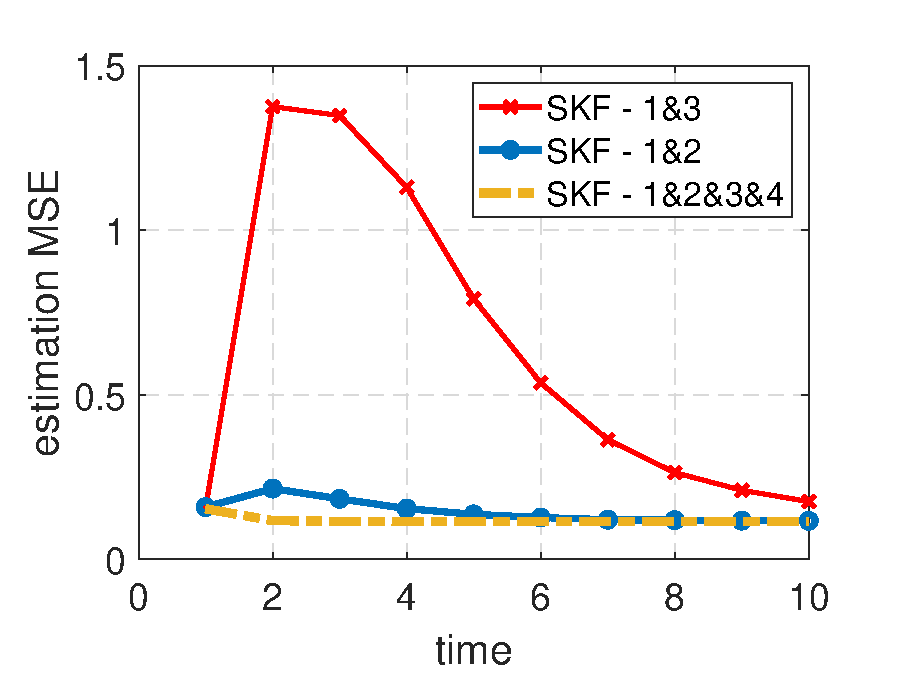
\includegraphics[width=0.35\textwidth]{error-diff.eps}
    %\label{fig:ex3}
    \caption{ The bimodal SKF using modes 1&2 has an estimation error very close to that of a 4-modal SKF.  }
    \label{fig:rmodal}
        \vspace{-0.4cm}
\end{figure}


\begin{figure}
  \centering
    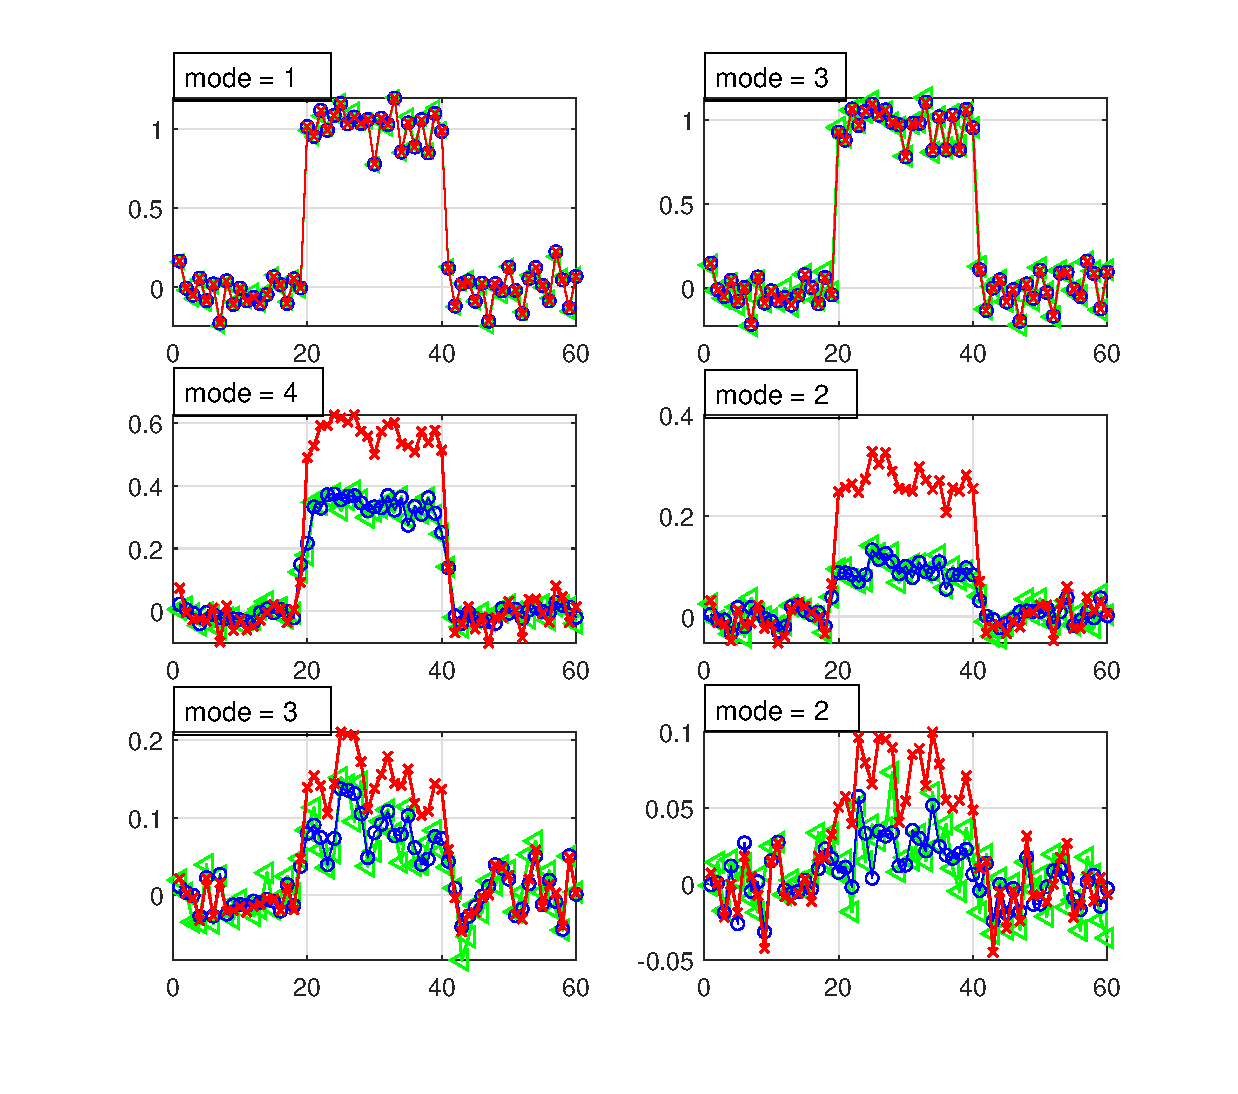
\includegraphics[width=0.5\textwidth]{realization.eps}
    %\label{fig:ex3}
    \caption{ One realization of state variables are plotted for 6 time step; the green shows the groundtruth signal, the blue is the bimodal using 1&2 and the red is the estimates using 1&3. }
    \label{fig:rmodal}
        \vspace{-0.4cm}
\end{figure}

It can be observed that replacing the 4-modal system with the bi-modal system including modes 1&3 induces a small estimation error but brings in a significant computational saving. We are able to quantify this induced estimation error using the proposed structure in the paper. The computations required in the 4-modal SKF and bimodal SKF correspond to running $4^r$ and $2^r$ Kalman filters, respectively (where $r$ is the number of previous time steps we assume to keep in the SKF approximation). The optimal representative of each cluster in this example can be approximated by $\frac{A_1+A_3}{2}$ and $\frac{A_4+A_2}{2}$, which result in an even smaller estimation error (the results are not included due to space restrictions). 
       
\section{Conclusion and future work}\label{section:con}
A novel graph-based representation for an SLDS is proposed. The nodes and edges of this graph are defined based on the parametric models of the SLDS. This graph structure is used to find the best set of modes to use in an estimator for the SLDS given an error tolerance. The benefit of this model is demonstrated in the simulations. Proposing a partially connected graph and use this algorithm to make online decisions in real time/batch system identification algorithms is a future work. 
\bibliography{mycite}{}
\bibliographystyle{IEEEtran}




% \section*{References}

% \subsection*{Basic format for books:}

% J. K. Author, “Title of chapter in the book,” in {\em Title of His Published Book}, xth ed. City of Publisher, (only U.S. State), Country: Abbrev. of Publisher, year, ch. x, sec. x, pp. xxx--xxx.

% \subsection*{Examples:}
% \def\refname{}
% \begin{thebibliography}{34}

% \bibitem{}G. O. Young, “Synthetic structure of industrial plastics,” in {\em Plastics}, 2nd ed., vol. 3, J. Peters, Ed. New York, NY, USA: McGraw-Hill, 1964, pp. 15--64.

% \bibitem{}W.-K. Chen, {\it Linear Networks and Systems}. Belmont, CA, USA: Wadsworth, 1993, pp. 123--135.

% \end{thebibliography}

% \subsection*{Basic format for periodicals:}

% J. K. Author, “Name of paper,” Abbrev. Title of Periodical, vol. x,   no. x, pp. xxx--xxx, Abbrev. Month, year, DOI. 10.1109.XXX.123--456.

\end{document}
